%------------------------------------------------
% main.tex - MA1500 2014-15
%------------------------------------------------
\documentclass{camel}
\usepackage{camel}

\academicyear{2014-15}
\modulecode{MA0000}
\moduletitle{Camel Theory}

\printanswersatend


\usepackage{graphicx}
%------------------------------------------------
\begin{document}

\chapter{Theorems}\label{ch:theorems}

\begin{theorem}
This is the statement of the theorem
\end{theorem}

\begin{proof}
xx

xx

xx

xx
\end{proof}

%\chapter{Cymraeg}\label{ch:cymraeg}
%
%\cym{Cymraeg yw hwn}
%
%\eng{This is English}

\chapter{Figures}\label{ch:figures}

Here is a figure.
\begin{figure}[htb]
\centering
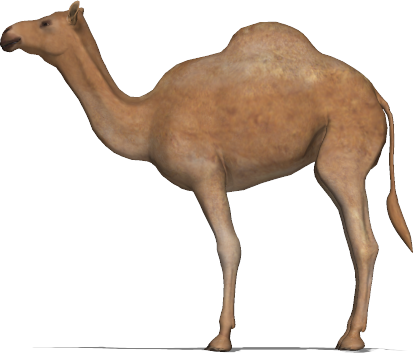
\includegraphics[scale=0.25]{figures/humpty.png}
\caption{Humpty the Camel.}
\label{humpty-the-camel}
\end{figure}
No more figures.

\chapter{Lists}\label{ch:lists}

Initial text.
\begin{itemize}
\item First item of list
\begin{enumerate}
\item First item of nested list.
\item Second item of nested list.
\end{enumerate}
\item Second item of list
\end{itemize}
Final text.

\chapter{Labels, References and Citations}

\begin{itemize}
\item Here we include a label: \label{ch:introduction}.
\item Here we include a reference: \ref{ch:introduction}.
\item Here we include a citation: \cite{video_ex.1.1.1}.
\end{itemize}

\chapter{Exercises}\label{ch:exercises}

\section{Written solutions}\label{se:written-solutions}

\begin{diagnostic}\label{diag:demo}
This is the introduction.
\begin{questions} 
\question This is the first question.\label{qu:first-question}
\begin{answer} 
This is the answer to the first question.
\end{answer} 
\question This is the second question.\label{qu:second-question}
\begin{answer} 
This is the answer to the second question.
\end{answer} 
\question This is the third question.\label{qu:third-question}
\begin{parts}
\part This is the first part of the third question
\begin{answer} 
This is the answer to the first part of the third question.
\end{answer} 
\part This is the second part of the third question
\begin{answer} 
This is the answer to the second part of the third question.
\end{answer} 
\end{parts}
\end{questions} 
\end{diagnostic}

%---------------------------------------
\section{Multiple choice}

% formative
\begin{formative}\label{di:beatles} 
Please complete the following formative exercise.
\begin{questions} 
\question Which is the odd one out?  
\begin{choices} 
\correctchoice Tom
\choice Paul 
\choice George 
\choice Ringo 
\end{choices} 
\question Which is the odd one out?  
\begin{choices} 
\choice John 
\correctchoice Ball 
\choice George 
\choice Ringo 
\end{choices} 
\end{questions}
\end{formative}

%---------------------------------------
\section{Other Exercises}

\begin{exercise}
Please complete the following optional exercise.
\begin{questions} 
\question Faint o'r gloch yw hi?
\end{questions}
\end{exercise}

\end{document}

